\documentclass{beamer}
\usepackage{ctex, hyperref}
\usepackage[T1]{fontenc}
\usepackage{amsmath,amssymb,xcolor,booktabs}
\usepackage{graphicx}
\usepackage{multicol}

\author{汇报人：董祉含}
\title{基于动态参考点的CPT-PG在线策略优化}
\subtitle{开题答辩}
\institute{上海财经大学统计与数据科学学院}
\date{2026年6月8日}
\usepackage{SUFE}

\definecolor{deepblue}{RGB}{18,58,105}
\definecolor{deepred}{RGB}{150,35,35}
\definecolor{deepgreen}{RGB}{24,111,80}
\definecolor{lightgray}{RGB}{245,247,250}

\newcommand{\key}[1]{\textcolor{deepred}{\textbf{#1}}}
\newcommand{\smallcap}[1]{\textcolor{deepblue}{\textbf{#1}}}

\begin{document}

\kaishu

\begin{frame}
    \titlepage
    \begin{figure}
        \centering
        
\includegraphics[width=0.38\linewidth]{pic/sufe.png}
    \end{figure}
\end{frame}

\begin{frame}{研究背景与研究现状}
    \scriptsize
    \begin{columns}[T]
        \begin{column}{0.49\textwidth}
            \begin{block}{研究背景}
                \begin{itemize}
                    \item 投资组合强化学习通常以期望收益或风险调整收益为目标。
                    \item 投资者评价盈亏时依赖心理参考点。
                    \item 累积前景理论（CPT）刻画损失厌恶、概率权重扭曲和参考点依赖。
                    \item 非平稳市场中，参考点随财富路径变化。
                \end{itemize}
            \end{block}
        \end{column}
        \begin{column}{0.47\textwidth}
            \begin{block}{研究现状}
                \begin{itemize}
                    \item CPT结合RL研究智能体识别人类行为偏好。
                    
                    \item 现有CPT-RL主要采用固定参考点和平稳环境设定。
                    \item 行为金融研究验证了参考点路径依赖和非对称适应。
                \end{itemize}
            \end{block}
        \end{column}
    \end{columns}
    \vspace{0.05em}
    \begin{block}{投资者的路径依赖和处置效应现象}

        \begin{itemize}
        \item 同样从初始财富1.0到1.2，持续上涨和先涨后跌会带来不同心理评价。终点相同，路径不同，参考点和风险态度也会不同。
        \item 投资者更早卖出盈利股票落袋为安，但对亏损股票持有更久，期待反弹。
        \end{itemize}
    \end{block}
\end{frame}

\begin{frame}{研究问题与本文价值}
    \footnotesize
    \begin{block}{核心研究问题}
        非平稳市场中，动态参考点变化时，DRCPT-PG能否稳定跟踪时变CPT目标函数的一阶驻点集合？
    \end{block}
    \vspace{0.35em}
    \begin{columns}[T]
        \begin{column}{0.48\textwidth}
            \begin{block}{理论意义}
                \begin{itemize}
                    \item 将CPT-PG从静态参考点推广到动态参考点。
                    \item 改良梯度更新方式，引入动态局部遗憾作为跟踪评估指标。
                    \item 基于因子得分的Dirichlet策略函数表达连续投资组合权重。
                \end{itemize}
            \end{block}
        \end{column}
        \begin{column}{0.48\textwidth}
            \begin{block}{实际价值}
                \begin{itemize}
                    \item 为智能体提供可解释、可控制的更贴近投资者心理的参数化框架。
                    \item 通过半合成实验，控制市场阶段切换和冲击，评估策略稳定性。
                    \item 通过半合成实验，验证智能体是否能表现出处置效应和路径依赖的人类行为。
                \end{itemize}
            \end{block}
        \end{column}
    \end{columns}
\end{frame}

\begin{frame}{研究框架}
    \centering
    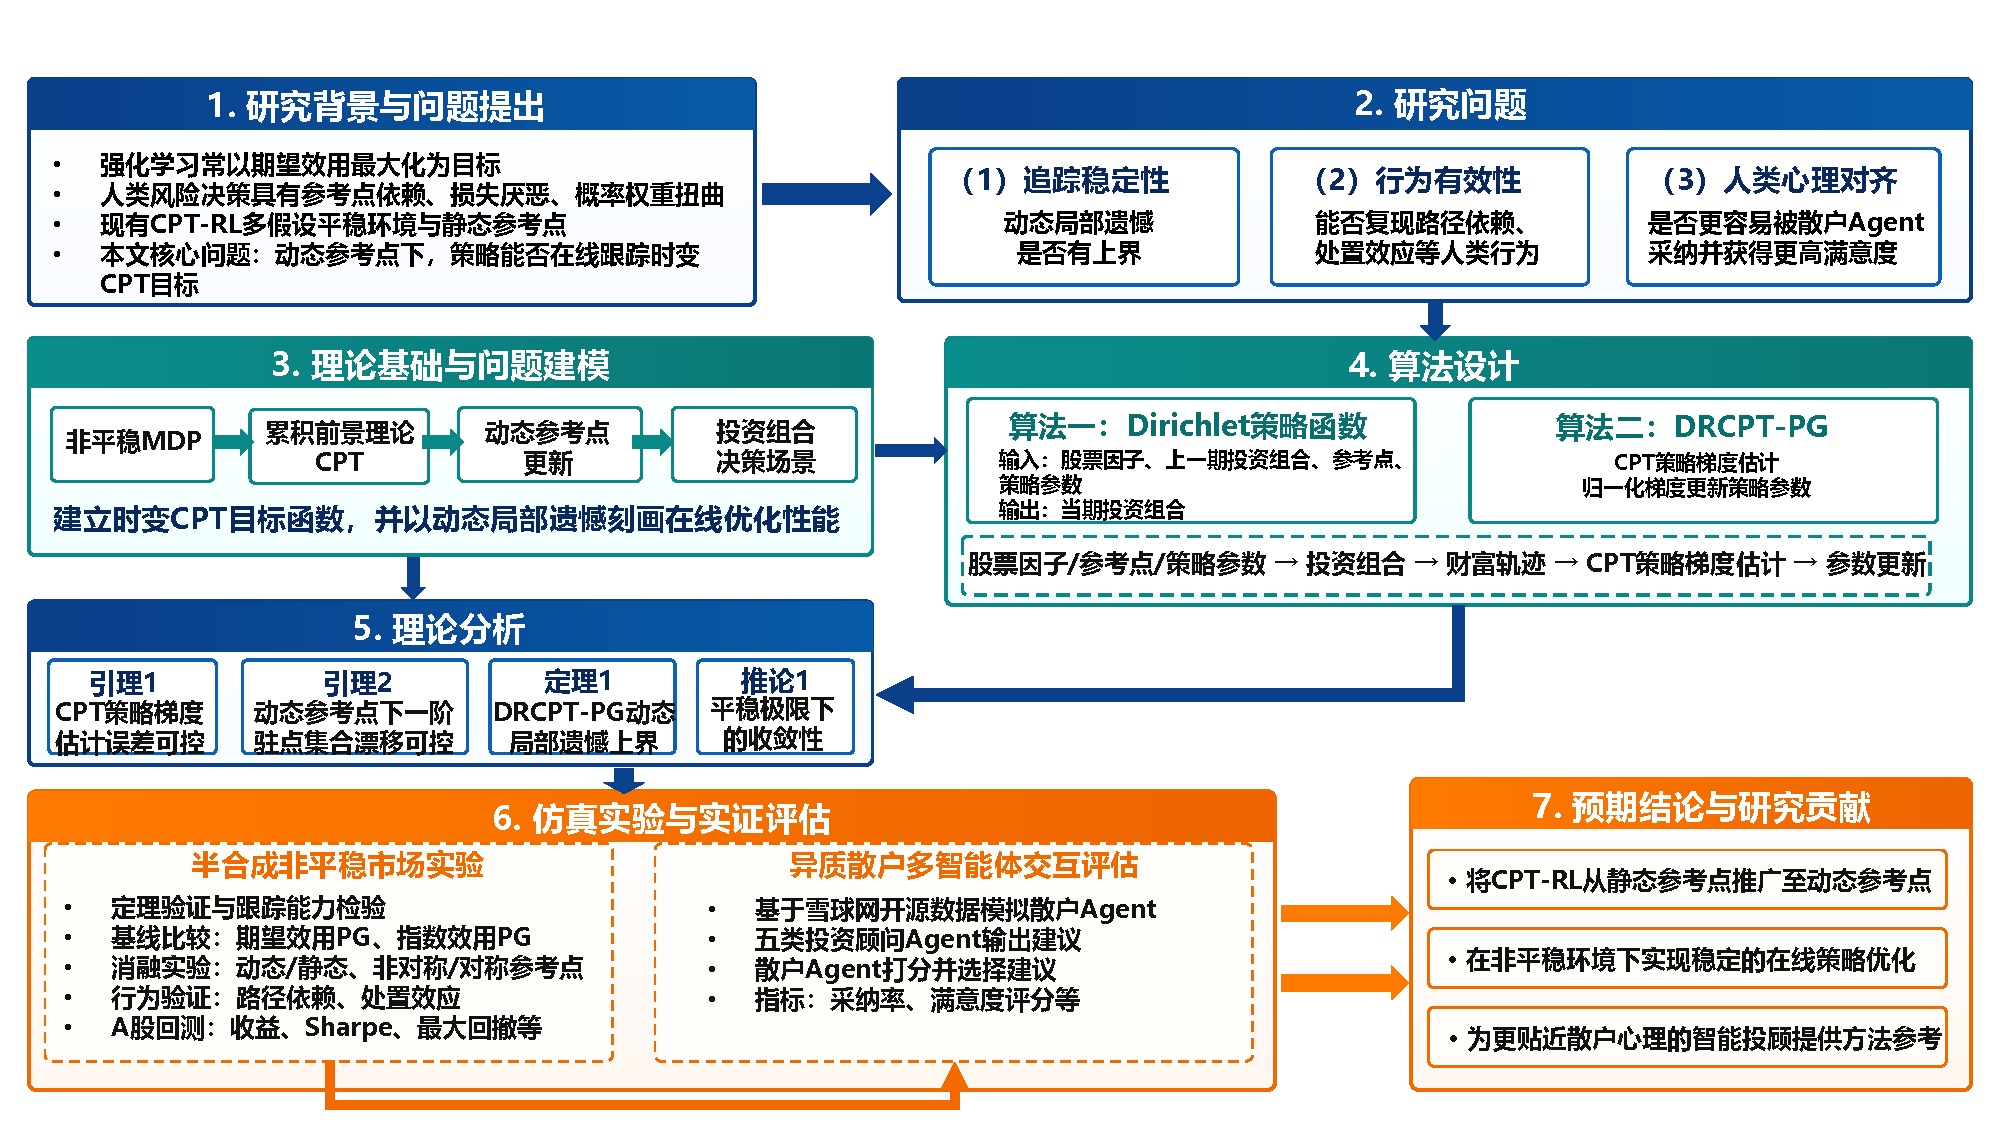
\includegraphics[width=0.96\linewidth,height=0.81\textheight,keepaspectratio]{pic/框架图.pdf}


\end{frame}

\begin{frame}{投资组合场景}
    \footnotesize
    \begin{columns}[T]
        \begin{column}{0.52\textwidth}
            \begin{block}{动作空间}
                第 $k$ 个时期起点为 $t_k$，$t_{k+1}=t_k+h$。时期内第 $u$ 天：
                \[
                a_u=(\omega_{0,u},\omega_{1,u},\ldots,\omega_{N,u})^\top
                \]
                \[
                \mathcal{A}=
                \left\{a\in \mathbb{R}^{N+1}:
                \sum_{i=0}^{N}\omega_i=1,\ \omega_i\ge 0
                \right\}
                \]
                $\omega_{0,u}$ 为现金权重，$i=1,\ldots,N$ 为风险资产。
            \end{block}
        \end{column}
        \begin{column}{0.44\textwidth}
            \begin{block}{动态参考点}
                \[
                \Delta_u=x_{u+1}-r_u
                \]
                \[
                r_{u+1}=
                \begin{cases}
                r_u+\eta_+\Delta_u, & \Delta_u\ge 0,\\
                r_u+\eta_-\Delta_u, & \Delta_u<0
                \end{cases}
                \]
            \end{block}
        \end{column}
    \end{columns}
    \vspace{0.4em}
    \begin{center}
        \smallcap{时期内逐日输出投资组合，并观测收盘后的财富更新参考点。}
    \end{center}
\end{frame}

\begin{frame}{数学问题：CPT目标、梯度估计与跟踪指标}
    \scriptsize
    \setlength{\abovedisplayskip}{2pt}
    \setlength{\belowdisplayskip}{2pt}
    \setlength{\jot}{1pt}
    \begin{columns}[T]
        \begin{column}{0.48\textwidth}
            \begin{block}{当期优化目标}
                财富轨迹 $\tau_{t_k}$ 的时期末财富为 $X_{t_k}$，逐日更新后的参考点为 $r_{t_k,h}$：
                \[
                Y_{t_k}(\tau_{t_k})
                =
                X_{t_k}(\tau_{t_k})-
                r_{t_k,h}(\tau_{t_k})
                \]
                \[
                J_{t_k}(\theta,r_{t_k})
                =
                \operatorname{CPT}
                \left(Y_{t_k}(\tau_{t_k})\right)
                \]
            \end{block}
            \begin{block}{梯度估计}
                \[
                \widehat{\nabla_\theta J}_{t_k}
                =
                \frac{1}{m_t}
                \sum_{j=1}^{m_t}
                \widehat{\phi}_{t_k,n_t}
                \!\left(Y_{t_k}^{(j)}\right)
                G_{t_k}^{(j)}
                \]
            \end{block}
        \end{column}
        \begin{column}{0.48\textwidth}
            \begin{block}{参数更新}
                \[
                \begin{aligned}
                \widehat{\overline{\nabla J}}_k
                &=
                \frac{1}{K}\sum_{i=0}^{K-1}
                \rho^i
                \widehat{\nabla_\theta J}_{t_{k-i}},\\
                K&=\sum_{i=0}^{K-1}\rho^i
                \end{aligned}
                \]
                \[
                \theta_{t_{k+1}}
                =
                \theta_{t_k}
                +\gamma
                \widehat{\overline{\nabla J}}_k
                \]
            \end{block}
            \begin{block}{跟踪指标}
                \[
                DLRegret(T/h)=
                \sum_{k=1}^{T/h}
                \|\widehat{\overline{\nabla J}}_{k}\|^2
                \]
            \end{block}
        \end{column}
    \end{columns}
\end{frame}

\begin{frame}{算法流程：DRCPT-PG在线优化}
    \centering
    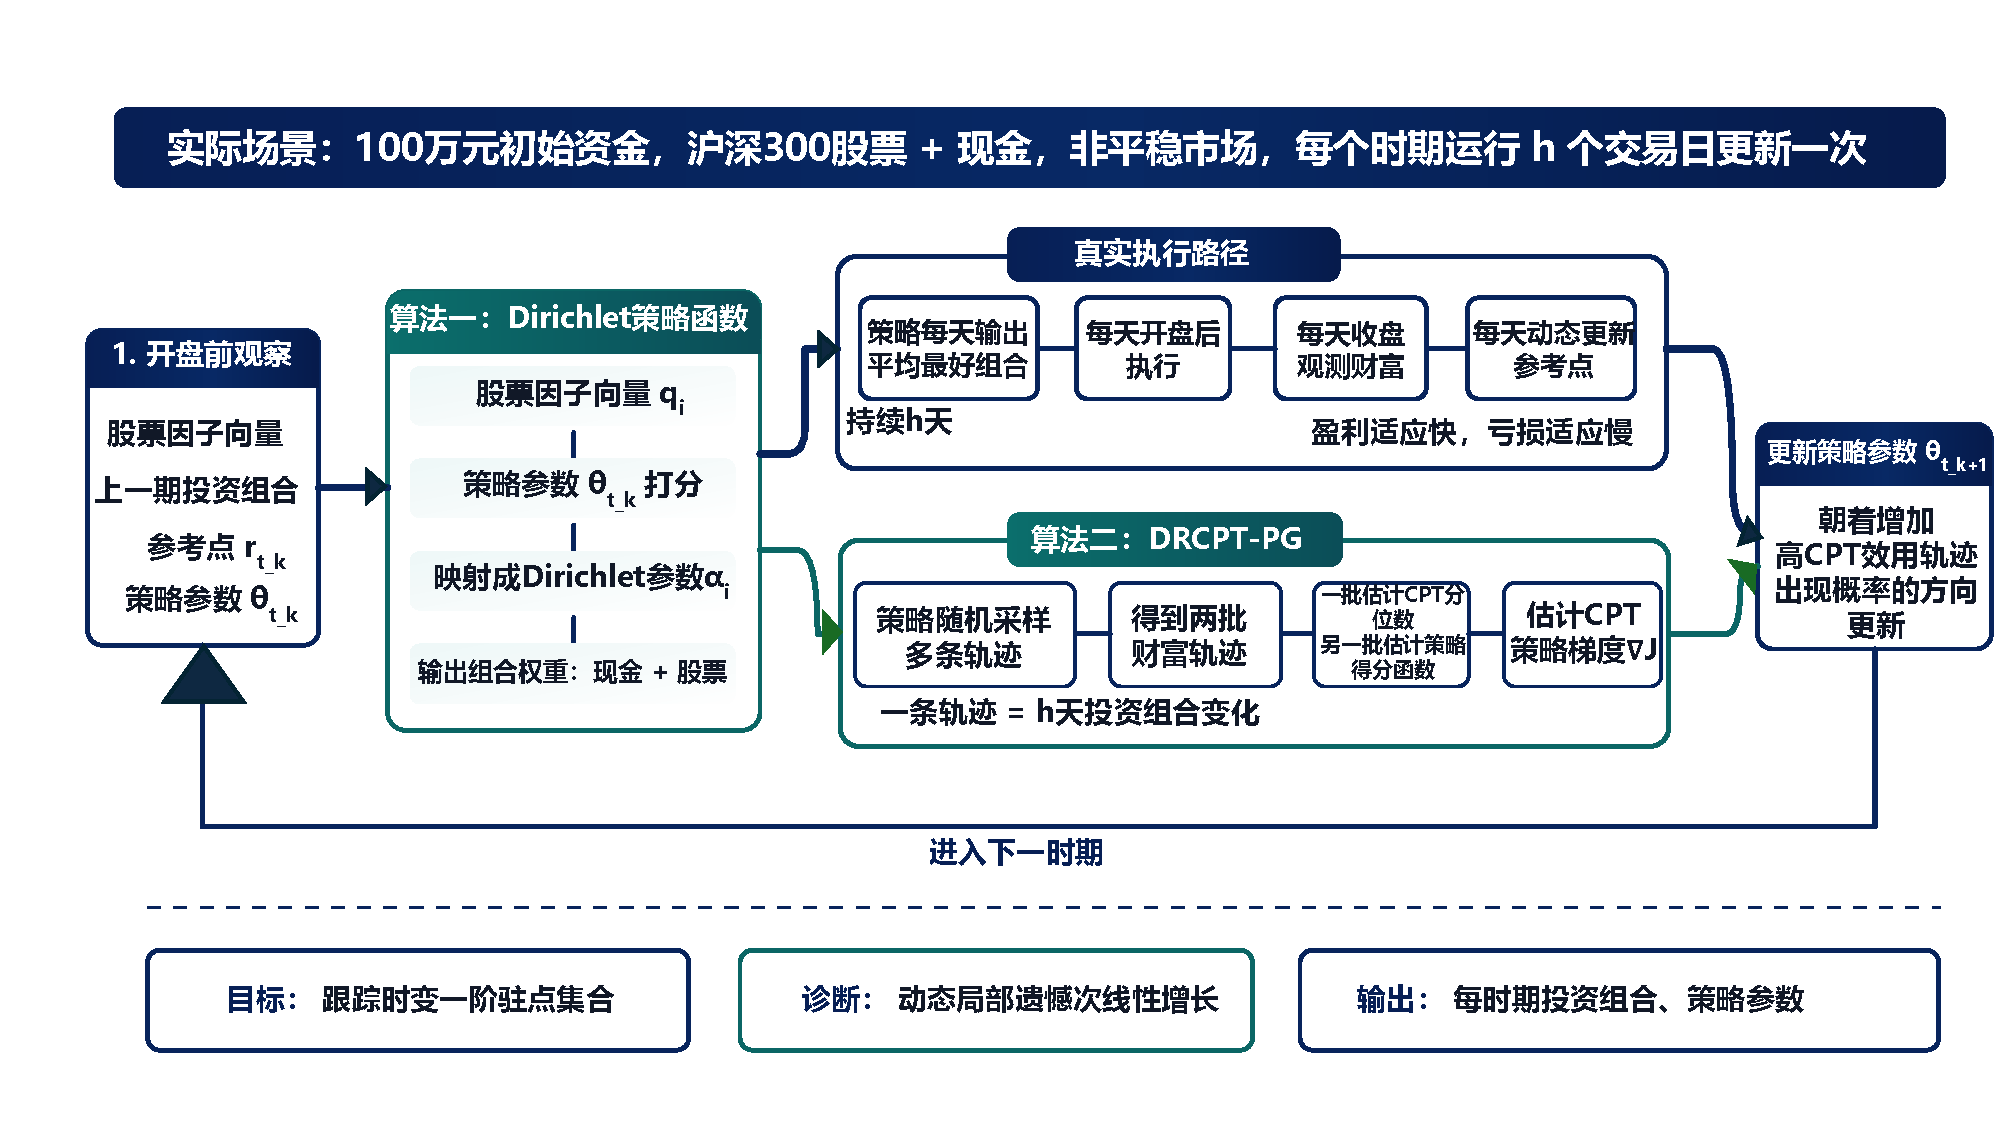
\includegraphics[width=0.96\linewidth,height=0.81\textheight,keepaspectratio]{pic/算法流程.pdf}
    
\end{frame}

\begin{frame}{数据来源与半合成机制}
    \footnotesize
    \begin{columns}[T]
        \begin{column}{0.48\textwidth}
            \begin{block}{数据来源}
                \begin{itemize}
                    \item 股票范围：沪深300成分股。
                    \item 市场数据：23-26年A股日频行情，包含OHLCV。
                    \item 因子构造：动量、反转、波动、质量、流动性等。
                    \item 清洗规则：剔除ST、退市和缺失字段严重的股票，并避免前视偏差。
                \end{itemize}
            \end{block}
        \end{column}
        \begin{column}{0.48\textwidth}
            \begin{block}{半合成机制}
                \begin{itemize}
                    \item 真实沪深300股票池，保留真实因子数据。
                    \item 收益由市场阶段和因子共同生成。
                    \item 设置上涨、震荡、市场冲击等阶段。
                    \item 考虑交易成本，根据调仓后财富扣除。
                \end{itemize}
            \end{block}
        \end{column}
    \end{columns}
    \vspace{0.15em}
    \begin{center}
        \key{作用：在真实因子基础上控制市场机制，使跟踪稳定性和人类行为更容易识别。}
    \end{center}
\end{frame}

\begin{frame}{当前进展：跟踪稳定性}
    \begin{columns}[T]
        \begin{column}{0.49\textwidth}
            \centering
            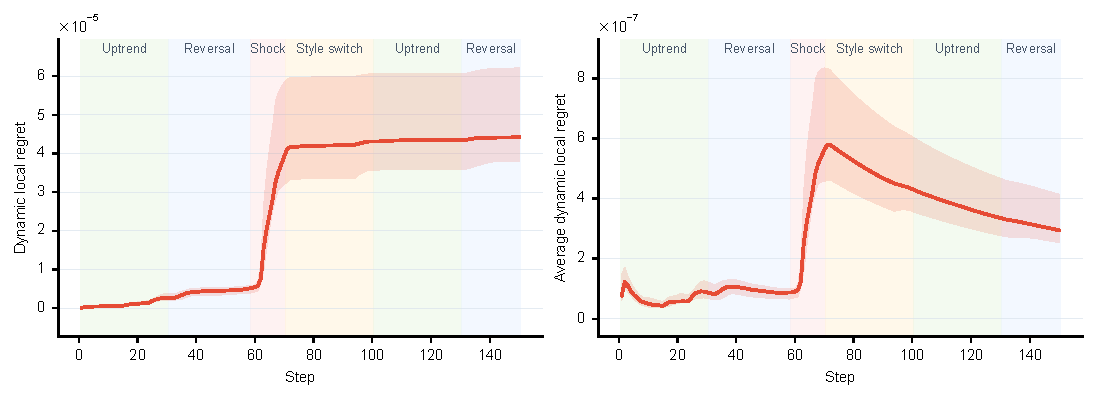
\includegraphics[width=\linewidth,height=0.65\textheight,keepaspectratio]{pic/nature_dynamic_reference_tracking.pdf}
            \scriptsize 动态参考点方法的动态局部遗憾
        \end{column}
        \begin{column}{0.49\textwidth}
            \centering
            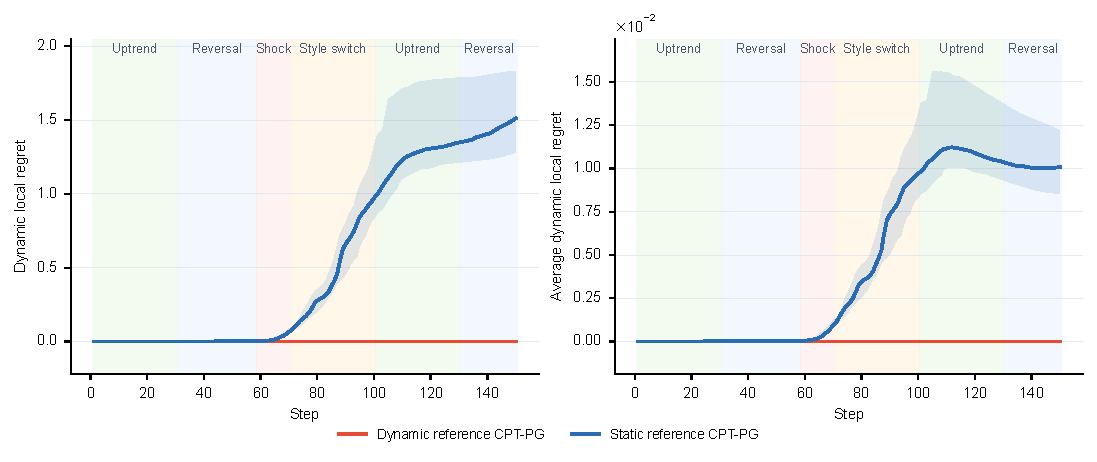
\includegraphics[width=\linewidth,height=0.58\textheight,keepaspectratio]{pic/nature_dynamic_static_tracking_comparison.pdf}
            \scriptsize 动态与静态参考点的跟踪对比
        \end{column}
    \end{columns}
    \vspace{0.5em}
    \small
    \begin{itemize}
        \item 动态参考点方法的动态局部遗憾保持在较低水平，表明算法能稳定跟踪时变CPT目标函数的一阶驻点集合。
        \item 市场冲击后，动态参考点方法的跟踪能力优于静态参考点方法，显示出更强的适应性和稳定性。
    \end{itemize}
\end{frame}

\begin{frame}{当前进展：多方法财富表现对比}
    \small
    \begin{block}{实验设置}
        半合成沪深300环境；资产池选择5股票+1现金；时期长度 $h=5$；固定步长 $\gamma=0.05$；固定采样轨迹数=256；重复运行10次；比较动态参考点CPT-PG、静态参考点CPT-PG、期望效用PG和指数效用PG。
    \end{block}
    \centering
    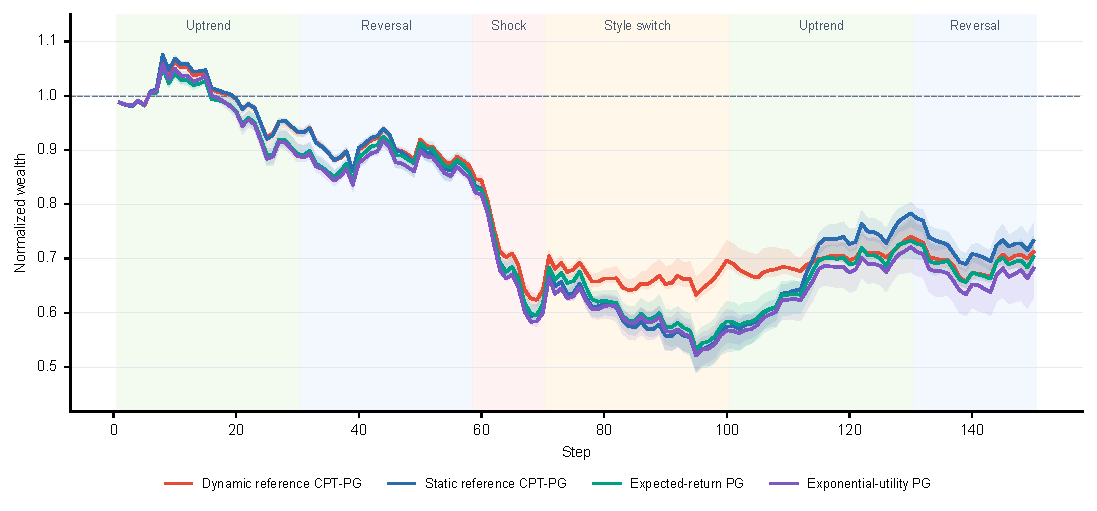
\includegraphics[width=0.94\linewidth,height=0.64\textheight,keepaspectratio]{pic/nature_four_method_wealth_regimes.pdf}

    \scriptsize
    图中背景色表示不同市场阶段，用于观察方法在阶段切换和市场冲击后的财富路径差异。
\end{frame}

\begin{frame}{后续安排}
    \small
    \begin{columns}[T]
        \begin{column}{0.31\textwidth}
            \begin{block}{6-7月}
                \begin{itemize}
                    \item 改良仿真实验。
                    \item 推进多智能体实验。
                    \item 撰写结果分析和结论。
                \end{itemize}
            \end{block}
        \end{column}
        \begin{column}{0.31\textwidth}
            \begin{block}{7-8月}
                \begin{itemize}
                    \item 检验理论分析的证明链路。
                    \item 核对假设、引理和定理之间的逻辑衔接。
                    \item 润色论文整体行文。
                \end{itemize}
            \end{block}
        \end{column}
        \begin{column}{0.31\textwidth}
            \begin{block}{9-10月}
                \begin{itemize}
                    \item 优化论文框架图和结果图。
                    \item 准备答辩文稿。
                    \item 润色答辩PPT。
                \end{itemize}
            \end{block}
        \end{column}
    \end{columns}

\end{frame}

\end{document}
